\documentclass[11pt]{article}

% Page geometry
\usepackage{geometry}
\geometry{
  margin=0.5in,% Equal margin of 0.5in from all four sides
  includefoot% Include only the footer in the margin calculations, since you don't have a header
}

% Header/footer
\usepackage{fancyhdr}
\pagestyle{fancy}% Page style will be fancy
\fancyhf{}% Clear headers and footers
\renewcommand{\headrulewidth}{0pt}% No header rule
%\renewcommand{\footrulewidth}{0pt}% No footer rule (default)
\fancyfoot[L]{Ryan D. Mueller} %\quad %\href{mailto:kathryn.haglin@appc.upenn.edu}{{\small kathryn.haglin@appc.upenn.edu}}}
\fancyfoot[C]{\textit{Cover Letter}}
\fancyfoot[R]{\thepage}

\usepackage{hyperref,graphicx}
\usepackage{color}
\setlength{\parindent}{0pt}% No paragraph indentation
\setlength{\parskip}{.5\baselineskip plus 0.1\baselineskip minus 0.1\baselineskip}

\begin{document}

%\includegraphics[width=2in]{TAM-PrimaryMarkA.png}% Logo
\hfill% FROM details
\begin{tabular}{@{}r@{}}
  \today \\
  [.5em]
Texas A\&M University \\
Physics and Astronomy Dept. \\
4242 TAMU \\
College Station, TX 77843-4242 \\
[.5em]
(651) 587-1581 \\
\href{mailto:rmueller@physics.tamu.edu}{rmueller@physics.tamu.edu}\\
%\href{http://khaglin.weebly.com/}{http://khaglin.weebly.com/}
\end{tabular}



\bigskip

% TO details
%\begin{tabular}{@{}l@{}}
%  Mrs.\ Jane Smith \\
%  Recruitment Officer \\
%  The Corporation \\
%  123 Pleasant Lane \\
%  City, State 12345
%\end{tabular}

% Rochester ------------------------------------------------
%\begin{tabular}{@{}l@{}}
% Department of Political Science \\
% University of Rochester \\
% Harkness Hall 333 \\
% Rochester, New York 14627-0146
%\end{tabular}
% -----------------------------------------------------------------------

% Emory ------------------------------------------------
%\begin{tabular}{@{}l@{}}
% Department of Political Science \\
% Emory University \\
% 327 Tarbutton Hall \\
% 1555 Dickey Drive \\
% Atlanta, GA 30322
%\end{tabular}
% -----------------------------------------------------------------------

% Brown ------------------------------------------------
%\begin{tabular}{@{}l@{}}
% Department of Political Science \\
% Brown University \\
% 36 Prospect Street \\
% Providence, RI 02912
%\end{tabular}
% -----------------------------------------------------------------------

% MIT ------------------------------------------------
%\begin{tabular}{@{}l@{}}
%Department of Political Science \\
% MIT \\
% E53-470 \\
% 77 Massachusetts Avenue \\
% Cambridge, MA 02139
%\end{tabular}
% -----------------------------------------------------------------------

% UMN ------------------------------------------------
\begin{tabular}{@{}l@{}}
School of Physics \& Astronomy \\
 University of Minnesota \\
116 Church Street S.E. \\
Minneapolis MN, 55455
\end{tabular}
% -----------------------------------------------------------------------


% McGill ------------------------------------------------
%\begin{tabular}{@{}l@{}}
%Department of Political Science \\
% McGill University \\
% Room 414, Leacock Building \\
%855 Sherbrooke Street West \\
%Montreal, Quebec H3A 2T7 \\
%\end{tabular}
% -----------------------------------------------------------------------

% UNC ------------------------------------------------
%\begin{tabular}{@{}l@{}}
%Department of Political Science \\
%The University of North Carolina at Chapel Hill \\
%361 Hamilton Hall, CB 3265 \\  
%Chapel Hill, NC 27599-326
%\end{tabular}
% -----------------------------------------------------------------------

% USC ------------------------------------------------
%\begin{tabular}{@{}l@{}}
%Department of Political Science \\
%University of Southern California \\ 
%3518 Trousdale Parkway \\
%Von Kleinsmid Center (VKC), Room 327 \\
%Los Angeles, CA 90089-0044
%\end{tabular}
% -----------------------------------------------------------------------

% UC Irvine ------------------------------------------------
%\begin{tabular}{@{}l@{}}
%Department of Political Science \\
%University of California, Irvine \\ 
%3151 Social Science Plaza \\
%Irvine, CA 92697-5100
%\end{tabular}
% -----------------------------------------------------------------------

% Boulder ------------------------------------------------
%\begin{tabular}{@{}l@{}}
%Department of Political Science \\
%University of Colorado, Boulder \\
%333 UCB \\
%Boulder, CO 80309-0333
%\end{tabular}
% -----------------------------------------------------------------------
% MSU ------------------------------------------------
%\begin{tabular}{@{}l@{}}
%Department of Political Science \\
%%Michigan State University \\
 %303 South Kedzie Hall \\
%East Lansing, MI 48824
%\end{tabular}
% -----------------------------------------------------------------------

% TCU ------------------------------------------------
%\begin{tabular}{@{}l@{}}
%Department of Political Science \\
%Texas Christian University \\
%2855 Main Drive \\
%Scharbauer Hall 2007 \\
%Fort Worth, TX 76129
%\end{tabular}
% -----------------------------------------------------------------------


% URI ------------------------------------------------
%\begin{tabular}{@{}l@{}}
%Department of Political Science \\
%University of Rhode Island \\
%206 Washburn Hall \\
% 80 Upper College Road \\
%  Kingston, RI 02881
%\end{tabular}
% -----------------------------------------------------------------------

% Purdue ------------------------------------------------
%\begin{tabular}{@{}l@{}}
%College of Liberal Arts \\
%Purdue University \\
%100 N.\ University St\\
%Beering Hall\\
%West Lafayette, IN 47907
%\end{tabular}
% -----------------------------------------------------------------------

% Penn State -------------------------------
%\begin{tabular}{@{}l@{}}
%Department of Political Science \\
%Penn State University \\
%203 Pond Lab \\
%University Park, PA 16802\\
%\end{tabular}
%  --------------------------------

% Emory -------------------------------
%\begin{tabular}{@{}l@{}}
%%Department of Political Science \\
%Emory University \\
%327 Tarbutton Hall \\
%1555 Dickey Drive \\
%Atlanta, GA 30322
%\end{tabular}
%  --------------------------------

% Georgia -------------------------------
%\begin{tabular}{@{}l@{}}
%Department of Political Science \\
%School of Public and International Affairs \\
%The University of Georgia \\
%302 Baldwin Hall \\
%Athens, GA 30602 \\
%\end{tabular}
%  --------------------------------



\bigskip

My research experience at CMS includes being the lead for a physics analysis, phenomenology work, development of new techniques, extensive service work on the muon systems, and 
leadership over new graduate students in the muon alignment group. I hope to continue looking for new, exotic particles and learning new skill sets at my next position, and I believe I would be a valuable member of the University of Minnesota team. 

In the next few pages, I've highlighted some aspects of my current research. 

BFF Z'

In my current research, we search for a novel Z' + associated b jet production at the LHC with the CMS experiment. This model is motivated by the recent lHCb discrepency observed in $R_K$ and $R_{K^{*}}$, representing the ratio of branching fraction of the decay of B mesons to muons and electrons, from the standard model prediction.  The anomoly in $R_K$ and $R_{K^{*}}$ combined with Belle's measurements nears 4$\sigma$[1]. This hint of lepton non-universality can be explained by the addition of a Z' particle which features a flavour changing $\delta_{bs}$ interaction, no coupling with lighter quarks, and no decay to first generation leptons. Because of it's unique couplings, we can search for the particle in conjunction with associated b-jets and probe lower mass points than other Z' analyses. Our main backgrounds are Drell-Yan (DY) (pair of high $p_T$ leptons with a jet from initial-state radiation (ISR) or some other process) and $t\bar{t}$ (2 b-jets and up to two leptons), with minor contributions from vector boson decays and single top events.  

 $R_{K^{*}} = \frac{B(B\rightarrow K^{*} \mu \mu)}{B(B\rightarrow K^{*} e e)}$
 
  $R_{K} = \frac{B(B^+\rightarrow K^+ \mu \mu)}{B(B\rightarrow K^+ e e)}$

Extending the work of Abdullah et al. [2], we design an optimal search strategy for 2016-2018 data from the CMS experiment. Possible Z' production mechanisms at the LHC feature a standard s-channel process, as well as a 1 and 2 associated b-jet case. The standard s-channel process is identical to the primary diagram in the inclusive search, and therefore gives us no extra advantage. So, in our search, we focus on the associated b-jet cases. The last case is dubbed "Bottom Fermion Fusion", in analogy to Vector Boson Fusion. Our events then feature paris of muons/b-jets in conjunction with 1 or two soft b-jets and low missing transverse energy (MET). 


\begin{figure}
    \centering
    $n_{SR}=n_{CR_{b}^{ee}}\frac{n_{CR_{no-b}^{\mu\mu}}}{n_{CR_{no-b}^{ee}}}$
    \caption{The basic equation for our data-driven background estimation. The ratio of the muon-anti-b region to the electron-anti-b region provides a scale factor, converting between electrons and muons. This multiplied by the count in the electron+}
    \label{fig:ABCD_eqn}
\end{figure}

\begin{figure}
    \centering
    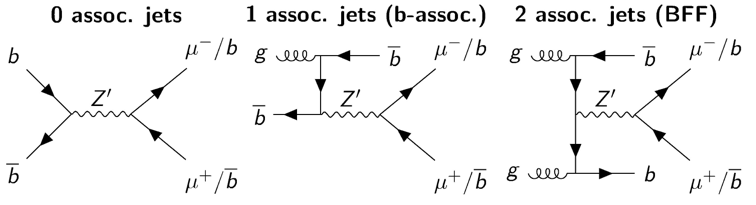
\includegraphics[width=\textwidth]{images/BFF_z_prime_cases.png}
    \caption{Z' production topologies at a hadron collider.}

    \label{fig:z_prime_cases}
\end{figure}


\begin{figure}
    \centering
    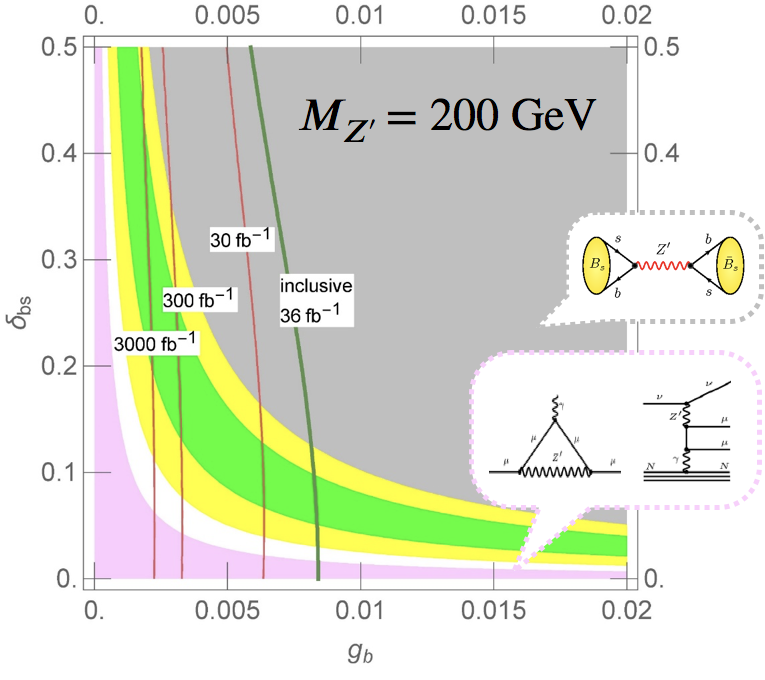
\includegraphics[width=8cm]{images/excluded_phase_space.png}
    \caption{Reach of b-associated Z' search at the LHC compared to the inclusive search. The top right grey area represents constraints from $B_s\rightarrow \bar{B}_s$ mixing, the bottom left represents constraints from neutrino trident production/g-2, and the green and yellow bands represent 1 and 2 standard deviation bands from the B anomalies. We see that the b-associated Z' search (red) excludes more phase space than the inclusive search (green).}
    \label{fig:exc_pahse_space}
\end{figure}


My search focuses on the muon channel, namely, where the Z' decays to two muons. Naturally, our search strategy selects for events featuring opposite sign muons and at least one b-jet. We also select for events featuring a pair of opposite sign electrons and jets not b-tagged for data-driven background estimation. Our sample is then divided into 1 and 2 jet bins. Three variables are used specially to reduce backgrounds. A $MET/M_{\ell\ell}$ (aka relative MET) filter takes advantage of the low transverse MET and high mass lepton pairs of the signal. Filtering on the difference between the hadronic transvers energy and letponic transvers energy (HT-LT) takes advantage of the fact that our associated b-jets tend to be "soft", or low energy. Finally, we permute the b-jets and leptons to create a best-guess top quark decay and compute it's mass (Top Mass Bound) to exclude top quarks from the final events. Cut values on these variables are optimized in monte-carlo simulation, and HT-LT and relative met cuts are optimized for variable mass points. 

At this point, data analysis is still a work in progress, but is scheduled to wrap up shortly. 

Muon Alignment

 Track based muon alignment is a critical task at CMS. The Alignment team is responsible for delivering up-to-date conditions of the positions of the muon detectors ensuring the muon system is operating optimally and developing further improvements to the muon alignment algorithm. I have contributed to nearly every aspect of track based muon alignment since joining CMS in 2014, from delivering conditions under tight deadlines to ensure proper data integrity, to leading group and inter-group investigations, teaching and guiding new members of muon alignment, and creating many new additions to muon alignment. 
 
 Some examples of my contributions include working with other members of the team to upgrade muon alignment in the DTs from 3 to 6 degrees of freedom, upgrading validation analysis code to function modularly and significantly faster, leading multiple investigations into systematic issues and developing a system to measure overall systematic measurements, creating a simplified standalone monte-carlo simulation of the muon alignment algorithm for educational purposes and for directed investigations into specific hard to investigate systematics, branching my toy mc simulation of muon alignment into a project for a new student, leading to an APS talk, guiding development of GEM alignment,  leading the group to reviving cosmic muon alignment, representing the Muon Alignment group at AlcaDB/DPG meetings and much more. Our work in recent years is currently being summarized in a new Muon Alignment note. I will bring my leadership and innovation demonstrated by my work in muon alignment to future research. 
 
 
 MonoTop:
 
 Certain exotic particles could result in single top production with right chirality at the LHC. Since standard model single top production are mostly left-chiral, if we can measure the chirality of the top quark, we can gain a better handle on these processes. I was part of a phenomenology project[3] developing a simple measure of chirality in top decays and a CMS analysis. 
 
 Traditional top chirality measurements are designed to work with $t\bar{t}$ events, requiring measurements between the lepton angles of both pair-produced top quarks. Our measurable relied on the relative energy difference between the b-jet and the lepton, allowing it to function independently of the top quark production mechanism. This not only made it useful for our monotop search, but also a general technique that could be applied to many top based analysis (e.g. precision standard model measurements).
 
This project has potential for further research. 


Trajectory:

At UMN, I 

 
 [1]https://link.springer.com/article/10.1007/JHEP01(2018)093
 
 
 [2]

@article{PhysRevD.97.075035,
  title = {Bottom-quark fusion processes at the LHC for probing ${Z}^{\ensuremath{'}}$ models and $B$-meson decay anomalies},
  author = {Abdullah, Mohammad and Dalchenko, Mykhailo and Dutta, Bhaskar and Eusebi, Ricardo and Huang, Peisi and Kamon, Teruki and Rathjens, Denis and Thompson, Adrian},
  journal = {Phys. Rev. D},
  volume = {97},
  issue = {7},
  pages = {075035},
  numpages = {7},
  year = {2018},
  month = {Apr},
  publisher = {American Physical Society},
  doi = {10.1103/PhysRevD.97.075035},
  url = {https://link.aps.org/doi/10.1103/PhysRevD.97.075035}
}

[3] source for monotop


[4] thin disk paper
the Run II inclusive search already excludes up to 2-4 TeV[1]
Dominant backgrounds: DY and TTbar
What do we offer over the inclusive search? 
Associated b-jet production greatly cuts through the background dominated < 500 GeV mass points
[1] https://doi.org/10.1007/JHEP06(2018)120


Neutrino Trident Production excludes bottom left
Bs->Bs mixing top right
Inclusive excludes high gb
Below ~350 GeV, we can probe new parameter spaces

Benefits of associate b-jet production

Produced b-jets are soft
low non-b-jet multiplicity
These two handles lets us greatly reduce DY and TTbar backgrounds

ABCD

$n_{SR}=n_{CR_{b}^{ee}}\frac{n_{CR_{no-b}^{\mu\mu}}}{n_{CR_{no-b}^{ee}}}$


\begin{table}[]
\begin{tabular}{lll}
Mass Point & z' Cross Section & Expected (35.9 fb\textasciicircum{}\{-1\} \\
200 GeV    & 0.289 pb         & $\sim$10k                                \\
350 GeV    & 0.031 pb         & $\sim$1k                                 \\
500 GeV    & 0.006 pb         & $\sim$230                                
\end{tabular}
\caption{BFF Z' production at the LHC.}
\end{table}



\bigskip

\begin{tabular}{@{}l@{}}
Sincerely, \\
  [.4em]
% \includegraphics[width=1.5in]{signature}\\ % my signature
  [.2em]
  Ryan D. Mueller
\end{tabular}
\end{document}




